\documentclass[hyperref,UTF8]{ctexart}
\usepackage[dvipdfmx]{graphicx}
\usepackage{gbt7714}
\usepackage{float}
\usepackage{ragged2e}
\usepackage{amsthm}
\usepackage{amssymb}
\usepackage{amsmath}
\usepackage{wrapfig}
\usepackage{tikz}
\usetikzlibrary{arrows.meta}
\usepackage{booktabs}
%\usepackage[a4paper,left=3.18cm,right=3.18cm,top=2.54cm,bottom=2.54cm]{geometry}
\usepackage{tabularx}
\usepackage{array}
\usepackage{caption}
\usepackage{hyperref}
\newcommand{\upcite}[1]{\textsuperscript{\textsuperscript{\cite{#1}}}}
\setCJKfamilyfont{song}{SimSun}
\newcommand{\D}{\mathrm{d}}
\title{讲义}
\author{赵翔}
\begin{document}
\maketitle
\section{万有引力和天体}
\subsection{从万有引力到开普勒三定律}
万有引力定律写成
\[F(r) = {GMm \over r^2}\]
要想得到加速度,要与$F=ma$结合,我们有
\[a(r) = {GM \over r^2}\]
这个关系是天体中最本质的关系,也是卫星运动的基本方程,注意这个加速度指向中心天体,我们想到如果这个天体的速度的大小和方向合适,那么可以做圆周运动,什么是合适的大小和方向?先让上面这个加速度等于圆周运动的向心加速度
\[{v^2 \over r} = {GM \over r^2}\]
可以解出
\[v = \sqrt{\frac{GM}{r}}\]
也就是说,当一个质点在$r$处时,必须以垂直于质点-天体连线为方向,以$\sqrt{\frac{GM}{r}}$为初速度大小发射时,质点\textbf{才能}做圆轨道运动,可见这种条件是十分苛刻的。好在,在我们的太阳系中,几大行星的轨道都十分接近正圆形。\\
\[
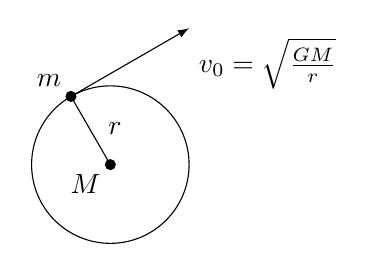
\begin{tikzpicture}
    \draw (0,0) circle (1cm);
    \fill (120:1) circle (2pt);
    \fill (0,0) circle (2pt);
    \node[below left] (O) at (0,0) {$M$};
    \node[above left] (A) at (120:1) {$m$};
    \node[below right] (A) at (60:2) {$v_0 = \sqrt{\frac{GM}{r}}$};
    \draw[-latex] (120:1)--(60:2);
    \draw (0,0)--(120:1);
    \node[above right] (O) at (120:0.3) {$r$};
\end{tikzpicture}
\]
\textbf{什么决定了天体的轨道?}

把一个质点在一个天体附近以一个初速度射出,那么它的轨道就是既定的,既然如此,就是先知道了初速度$v_0$和距离$r$,那么我们就不应该不分青红皂白的写向心力方程,我们应该沿着物理学基本的寻找守恒量的观点,
去寻找质点在只收万有引力作用下的守恒量,这个量可以从数学上推导出来,人们发现,在一个只受有心力\footnote{不止是万有引力,凡是受力方向始终指向一点均可}的系统中,下面的量是守恒的($v_\theta$是垂直于受力方向的速度分量,称为切向速度)
\[v_{\theta}r = {r^2\Delta \theta \over \Delta t} = {\Delta S \over \Delta t}\]
即单位时间扫过的面积,我们称之为掠面速度,掠面速度守恒就是开普勒第二定律的主要内容。
\begin{figure}[H]
    \centering
    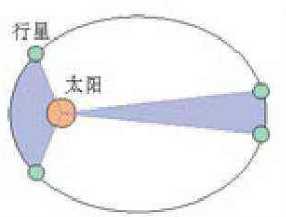
\includegraphics[width=3cm]{掠面速度.png}
    \caption{行星与太阳的连线在相等的时间扫过相等的面积}
\end{figure}
通过掠面速度守恒和万有引力定律,我们可以得出行星的轨道是一个椭圆,中心天体处在这个椭圆的一个焦点上,即开普勒第一定律,想要证明这一点并非易事,Feynman曾有一个巧妙的证明\footnote{参见\url{https://www.bilibili.com/video/BV1Zs411A7KJ?from=search&seid=6802919749265632960}},我们这里不过多介绍。

我们来对绕天体做半径为$R$圆轨道的卫星的周期做一些推导,周期$T$满足
\[T^2 = (\frac{2\pi R}{v})^2=\frac{4\pi^2 R^3}{GM}\]
于是
\[\frac{T^2}{ R^3} = \frac{4\pi^2}{GM}\]
在椭圆轨道中也有类似的结果,不过需要把$R$换成半长轴$a$
\[\frac{T^2}{a^3} = \frac{4\pi^2}{GM}\]
这就是开普勒第三定律,半长轴的三次方和周期的二次方成正比,由表达式还可看出,这个比值只于中心天体的质量有关。这个也是一个守恒量,不过要在多个卫星绕同一天体运行时才起作用,上面的掠面速度守恒则适用同一卫星运行时的不同位置时。

\subsection{宇宙速度}
我们在地球上抛出一个物体时,它做什么轨道运动,我们学过抛体运动,知道它将做抛物线运动,但是事实果真如此吗?抛出的苹果和天上的月亮会出现不同的轨道吗?

事实上,无论是抛出的苹果,还是天上的月亮,都在做椭圆轨道运动,只不过抛出的苹果速度太小,椭圆的半长轴太大(要想到另外一个焦点是地球中心),这个椭圆是如此之扁以至于它无论如何都会返回地面,而这一小部分运动轨迹就看起来像抛物线一样(图中这个椭圆还不够扁)
\[
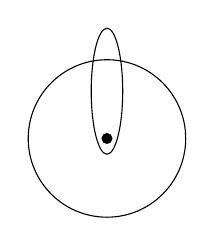
\begin{tikzpicture}
    \draw (0,0) circle (1cm);
    \draw (0,0.6) ellipse (0.2cm and 0.8cm);
    \fill (0,0) circle (2pt);
    \node[below left] (O) at (0,0) {};
\end{tikzpicture}
\]
所以,如果在地球附近沿切线射出一个物体,不考虑其它因素,如果速度合适,那么这个物体就可以绕地球(在地表附近)做圆轨道运动,这个速度也是发射卫星的最小速度,我们让上面的圆轨道条件中的$r$替换成地球半径$R$,我们得到了这个速度
\[v_1 = \sqrt{\frac{GM}{R}}=7.9 \mathrm{km}/\mathrm{s}\]
称为\textbf{第一宇宙速度}

那么既然能在地球附近做轨道运动,我们在航天上更关心,它速度达到多大时,可以脱离地球引力的束缚,这时就有了\textbf{第二宇宙速度}

为了介绍第二宇宙速度,我们先给出引力势能的概念\footnote{这部分仅作了解},引力势能与电势能类似,在无穷远初为0,越靠近中心天体越小,所以正常情况下这个势能为负
\[E_p = -\frac{GMm}{r}\]
其中$r$是到中心天体中心的距离,那么根据机械能守恒,我们出发点在地球表面,初速度是$v_0$,总能量是
\[\frac12 mv^2_0-\frac{GMm}{R}\]
在逃离中心引力场的束缚时,动能不断变为引力势能,如果将全部动能用完也还没能抵消完全势能,那么就无法脱离引力的魔爪,但要是引力势能变为0时(即无穷远),动能还有剩余,此时的总能量大于0,那么就是成功脱离了引力的束缚,于是我们只需要让总能量大于0,就是脱离的条件,即
\[\frac12 mv^2_0-\frac{GMm}{R} \geqslant   0 \]
解得
\[v_0\geqslant \sqrt{\frac{2GM}{R}}\]
右边的速度就是最小速度,即第二宇宙速度,也叫逃逸速度
\[v_2 = \sqrt{\frac{2GM}{R}} = 11.2 \mathrm{km}/\mathrm{s}\]

脱离太阳的引力要复杂的多,这里径直给出结论
\[v_3 = 16.7\mathrm{km}/\mathrm{s}\]
\subsection{引力半径和黑洞}
由逃逸速度的表达式可知,恒星质量越大,半径越小,逃逸速度越大,我们知道宇宙中的速度极限是光速,那么有没有逃逸速度是光速的天体呢?我们来推导一下这种天体应该满足的条件
\[v_2= c = \sqrt{\frac{2GM}{R}}\]
于是
\[R = \frac{2GM}{c^2}\]
这个半径称为\textbf{施瓦西半径},也叫引力半径,天体半径小于这个半径的天体叫\textbf{黑洞}
\end{document}